%%%%%%%%%%%%%%%%%%%%%%%%%%%%%%%%%%%%%%%%%%%%%%%%% PREAMBLE %%%%%%%%%%%%%%%%%%%%%%%%%%%%%%%%%%%%%%%%%%%%%%%%%%

%environment setup
\documentclass[letterpaper,11pt]{article}
\usepackage[square,comma,numbers,sort&compress]{natbib}
\bibliographystyle{ieeetr}
\usepackage{amsmath}
\usepackage{graphicx}
\usepackage{url}
\usepackage{xspace}
\usepackage[left=20mm,top=20mm]{geometry}
\usepackage{hyperref}
\usepackage{lineno}
\renewcommand{\familydefault}{\sfdefault}

%macros
\newcommand{\reffig}[1]{Figure~\ref{#1}}
\newcommand{\reftab}[1]{Table~\ref{#1}}
\newcommand{\refeq}[1]{Equation~\ref{#1}}
\newcommand{\refsec}[1]{Section~\ref{#1}}
\DeclareMathOperator*{\argmin}{arg\,min}
\newcommand{\Iota}{\mathrm{I}}

%%%%%%%%%%%%%%%%%%%%%%%%%%%%%%%%%%%%%%%%%%%% TITLE AND ABSTRACT %%%%%%%%%%%%%%%%%%%%%%%%%%%%%%%%%%%%%%%%%%%%%

%title
\title{Correcting Image Illumination for Differences in Exposure Time}
\author{Maggie Eminizer\\ \url{margaret.eminizer@gmail.com}\\ JHU Astropath Group}
\date{\today}
\begin{document}
\maketitle

%start numbering lines
\linenumbers

%abstract
\abstract{}

%%%%%%%%%%%%%%%%%%%%%%%%%%%%%%%%%%%%%%%%%%% INTRODUCTION SECTION %%%%%%%%%%%%%%%%%%%%%%%%%%%%%%%%%%%%%%%%%%%%
\section{Introduction}
\label{sec:introduction}

An important step in preparing a protocol for scanning a set of fluorescent tissue sample slides using the Akoya Biosciences Vectra 3.0 or Vectra Polaris digital microscopy systems is specifying the amount of time for which the sample should be exposed to the camera \cite{vectra_user_manual,polaris_user_manual}. The exposure times specified in the protocol are chosen by referencing one or more example tissue regions and making sure the resulting images are sufficiently exposed to show structures of interest yet not saturated so that important details become washed out. One exposure time value is chosen per filter cube, each of which corresponds to several layers of the multiplexed images.

The microscopes also include a software feature called ``saturation protection,'' recommended to be included in every scanning protocol, that automatically adjusts the exposure time of individual high-power fields (HPFs) to prevent them being overexposed due to a greater-than-expected amount of fluorescence, bright dust on the slide, or any other reason \cite{vectra_user_manual,polaris_user_manual}. Therefore, while a scanning protocol does specify a \textit{maximum} exposure time for each broadband filter region, that maximum time is not reached in every case, and the actual exposure times of each image layer group can vary independently between HPFs on the same slide (or between slides). 

An example of exposure time variation is shown in \reffig{fig:exposure_time_variation_M9_1} for different layers of HPFs in the sample called \texttt{M9\_1}. The exposure times for image layers corresponding to the DAPI and Texas Red filter groups are different for many images in the sample, while the exposure times for image layers corresponding to the FITC and Cy3 filter groups are almost always the same with a few exceptions, and the layers corresponding to the Cy5 filter group were all exposed for the same amount of time. The variations for layers of this sample in particular are very visible, though not entirely atypical.

\begin{figure}[!ht]
\centering
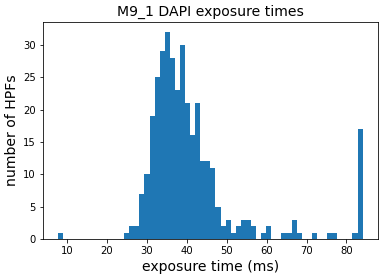
\includegraphics[width=0.3\textwidth]{images/introduction/exposure_times_M9_1_layer_1}
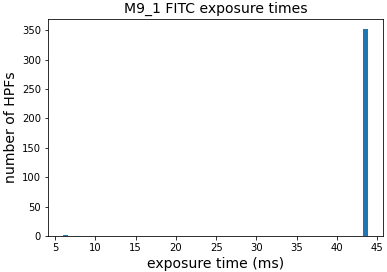
\includegraphics[width=0.3\textwidth]{images/introduction/exposure_times_M9_1_layer_10}
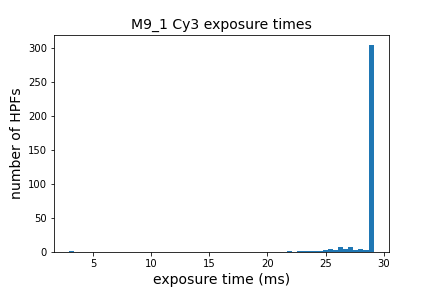
\includegraphics[width=0.3\textwidth]{images/introduction/exposure_times_M9_1_layer_19}
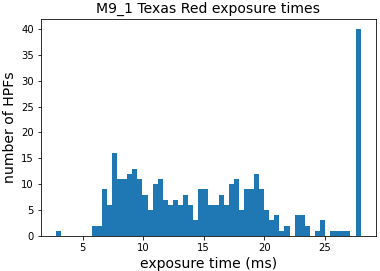
\includegraphics[width=0.3\textwidth]{images/introduction/exposure_times_M9_1_layer_26}
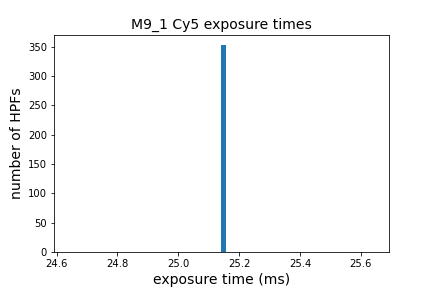
\includegraphics[width=0.3\textwidth]{images/introduction/exposure_times_M9_1_layer_33}
\caption{\footnotesize Exposure times for different layers of HPFs in the dataset \texttt{M9\_1}. Shown from top left to bottom right are layers 1, 10, 19, 26, and 33, respectively, corresponding to the first layers in each of the DAPI, FITC, Cy3, Texas Red, and Cy5 filter groups, respectively. The DAPI and Texas Red layers show substantial variation in exposure time, while the FITC and Cy3 layers show less variation for this sample, and the Cy5 layers of every HPF were all recorded with the same exposure time.}
\label{fig:exposure_time_variation_M9_1}
\end{figure}

Two example image layers with the minimum and maximum exposure times in the FITC filter group for this sample are shown in \reffig{fig:max_min_M9_1_fitc_images} to illustrate the behavior of the saturation protection feature. The minimally-exposed image layer clearly shows the single bright spot that triggered the saturation protection, stopping exposure of that HPF layer before it could be completely washed out by the noise from the spot. The maximally-exposed image layer shows no such localized brightness, and so it was exposed for the full, maximum time specified in the protocol.

\begin{figure}[!ht]
\centering
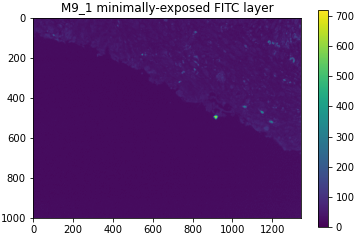
\includegraphics[width=0.45\textwidth]{images/introduction/min_exposure_M9_1_fitc_image}
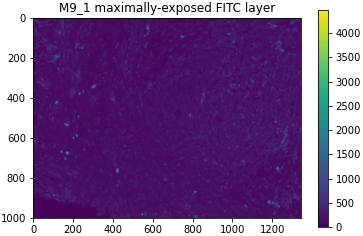
\includegraphics[width=0.45\textwidth]{images/introduction/max_exposure_M9_1_fitc_image}
\caption{\footnotesize Example images in layer 11 (corresponding to the FITC filter group) in the dataset \texttt{M9\_1} with the minimum (left) and maximum (right) recorded exposure time. The image layer with the minimum exposure time shows a clear bright spot that triggered the saturation protection feature in the Vectra 3.0 microscope software.}
\label{fig:max_min_M9_1_fitc_images}
\end{figure}

But comparing the actual numbers of counts in these image layers shows a challenge that arises from curtailing the exposure of some HPF layers. In the HPF whose FITC layers were exposed for the full, maximum time of 43.8 ms, the fluorescent tissue regions often register over a thousand counts, but the fluorescent tissue visible in the HPF layer exposed for the minimum time of 6.0 ms rarely registers more than a couple hundred counts. While a visual comparison is easily made for a human observer who can recognize that the minimally-exposed image layer shows some dark background, some tissue, and a bright spot, a quantitative comparison of the image counts themselves would not necessarily lead to the same conclusion.

Another way in which exposure time settings and the saturation protection feature can complicate analysis happens when the maximum exposure time is set too high for the typical tissue in the specimen. When the maximum exposure time is too high, most images saturate and are recorded with some smaller, often unique exposure time, like what is seen in the DAPI layer for the \texttt{M9\_1} sample. Two example image layers with the median and maximum exposure times in the DAPI filter group for the \texttt{M9\_1} sample are shown in \reffig{fig:med_min_M9_1_dapi_images}. In this case, the epiethilial tissue visible in the image layer with the maximum exposure time (84.0 ms) is relatively dim, but most DAPI layers in the sample show the much brighter cells that are visible in the example image layer with the median exposure time (38.0 ms). When this even greater amount of variation is observed for a group of sample layers, the result is a large number of images whose numbers of counts do not directly translate to the brightness of the fluorescent tissue at each location within the sample.

\begin{figure}[!ht]
\centering
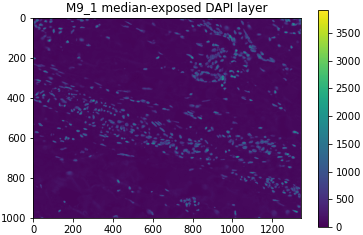
\includegraphics[width=0.45\textwidth]{images/introduction/med_exposure_M9_1_dapi_image}
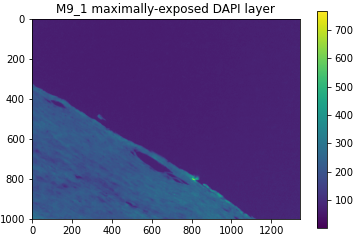
\includegraphics[width=0.45\textwidth]{images/introduction/max_exposure_M9_1_dapi_image}
\caption{\footnotesize Example images in layer 1 (corresponding to the DAPI filter group) in the dataset \texttt{M9\_1} with the median (left) and maximum (right) recorded exposure times. The image layer with the median exposure time shows typically-illuminated cells that were interpreted as bright spots by the saturation protection feature after the maximum exposure time was set using the relatively much dimmer epithelial tissue visible in the image layer with the maximum exposure time.}
\label{fig:med_min_M9_1_dapi_images}
\end{figure}

Differences in exposure time can be simply compensated for by considering counts per unit time rather than total counts, and the inForm and Phenochart softwares both offer ``normalized for exposure'' analysis modes that do exactly that \cite{inform_user_manual,phenochart_user_manual}. While this simple correction may be effective for qualitative or visual analysis of images, it is not sufficient for highly automated and quantitative analyses that rely on image data being as accurate and consistent as possible across large numbers of independent samples. 

A more sophisticated model applies corrections that are still linear, in that the number of counts collected increases proportionally to the total exposure time, but with an important offset for a small number of counts, called the ``dark current,'' representing noise in the camera that is present regardless of exposure to fluorescent tissue. This small, time-independent dark current is determined almost entirely by the gain, readout noise, and DC offset of the camera used to collect the microscopy images \cite{doi:10.1111/j.1365-2818.2011.03581.x}, and including it in the linear correction model is especially important for dim images whose true signal content may be comparable to the small noise in the first place.

The structure of this note is as follows. \refsec{sec:methods} describes the methods developed and the data used to measure the dark current offset as a function of image layer using portions of tissue that are multiply imaged in an overlapping fashion. \refsec{sec:results} details the results of the investigations, and the impact that applying the correction model has to finding layer-dependent thresholds for background illumination. \refsec{sec:summary} gives a brief summary.

%%%%%%%%%%%%%%%%%%%%%%%%%%%%%%%%%%%%%%%%%%%%%% METHODS SECTION %%%%%%%%%%%%%%%%%%%%%%%%%%%%%%%%%%%%%%%%%%%%%%
\section{Methods}
\label{sec:methods}

\subsection{General procedure}
\label{ssec:general_procedure}

When a slide is automatically scanned using the Vectra 3.0 or Vectra Polaris systems, an initial overview image is first collected at low magnification to determine where the tissue of interest is located within the slide. The microscope software then determines a rectangular grid overlaid on that tissue region, where each rectangle is a single HPF that must be collected so that the entire tissue region can be imaged at high magnification. The grid of HPFs is arranged with 20\% overlap between adjacent fields, meaning that some portions of the slide are imaged multiple times. These multiply-imaged ``overlap'' regions are used in a number of analyses to improve the quality of the overall composite high-magnification image, including registering individual HPF locations into a global coordinate system with sub-pixel accuracy, as discussed in~\cite{Heshy}.

Sometimes, two overlapping HPFs are recorded with different exposure times. When this happens, both image regions show identical content (within some caveats discussed below) at different scales of illumination. One such example of an overlap where the individual HPF image layers were recorded with difference exposure times is shown in \reffig{fig:raw_M9_1_overlap_66}, for the 66th overlap in the \texttt{M9\_1} sample. The comparison shows that the two image regions have contain similar content in substance, but at slightly different scales of illumination due to the differences in exposure times. 

\begin{figure}[!ht]
\centering
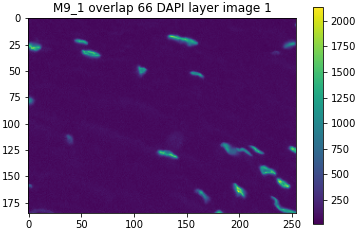
\includegraphics[width=0.49\textwidth]{images/methods/raw_M9_1_overlap_66_dapi_image_1}
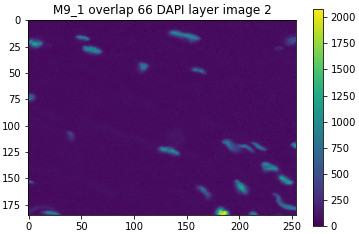
\includegraphics[width=0.49\textwidth]{images/methods/raw_M9_1_overlap_66_dapi_image_2}
\caption{\footnotesize First layer of the 66th overlap region in the \texttt{M9\_1} sample. The left image shows the lower left corner of an HPF whose first layer was exposed for 35.0 ms, and the right image shows the upper right hand corner of an adjacent HPF whose first layer was exposed for 30.0 ms.}
\label{fig:raw_M9_1_overlap_66}
\end{figure}

If the total number of counts recorded at a given pixel is modeled as some constant number of dark current counts, plus some number of counts from the fluorescent tissue that increases proportional to the amount of time the tissue is exposed to the camera, the dark current can be determined by minimizing the difference of the two HPF contents within the overlapping region.

To illustrate this concept more explicitly, consider two image regions $I^{ijm}_{1}$ and $I^{ijm}_{2}$, represented as three-dimensional tensors whose contents are the number of counts recorded by the camera and the $i=1, \ldots, H$, $j = 1, \ldots, W$, and $m = 1, \ldots, L$ indices range over the height ($H$ pixels), width ($W$ pixels), and number of image layers $L$, respectively, of the overlap region in question. If the two HPFs of which $I_{1}$ and $I_{2}$ are subsets are recorded with layer-dependent exposure times $t^{m}_{1}$ and $t^{m}_{2}$, respectively, then the number of counts at each pixel can be modelled linearly as
\begin{equation}
I^{ijm}_{1} = D^{m} + F^{ijm} t^{m}_{1} \hspace{0.08\textwidth} \mathrm{and} \hspace{0.08\textwidth} I^{ijm}_{2} = D^{m} + F^{ijm} t^{m}_{2},
\end{equation}
where $D^{m}$ is the constant number of counts from the dark current in the given image layer, and $F^{ijm}$ represents the luminous flux (in counts per unit time) of the underlying fluorescent tissue that is incident on each pixel at each wavelength. Note that while the dark current should, theoretically, be the same in each image layer, the actual noise may vary over time as the multiply-stained samples are successively illuminated at different wavelengths of light, and so we measure the number of dark current counts independently in each image layer.

Because the true $F^{ijm}$ are unknown, the numbers of dark current counts must be estimated a-posteriori. To that end, for arbitrary dark current offsets $D^{m}$, we define $\Iota^{ijm}_{1}$ and $\Iota^{ijm}_{2}$, the overlapping image regions corrected to the same sample-median exposure times $t^{m}_{\mathrm{med}}$, as
\begin{equation}
\Iota^{ijm}_{1} = 
\begin{cases} 
      D^{m}+\left(\frac{t^{m}_{\mathrm{med}}}{t^{m}_{1}}\right)\left(I^{ijm}_{1}-D^{m}\right) & S_{ijm} I^{ijm}_{1} > D^{m}  \\
      I^{ijm}_{1} & I^{ijm}_{1} \leq D^{m} 
\end{cases}
\label{eq:image_corr_def_1}
\end{equation}
and
\begin{equation}
\Iota^{ijm}_{2} = 
\begin{cases} 
      D^{m}+\left(\frac{t^{m}_{\mathrm{med}}}{t^{m}_{2}}\right)\left(I^{ijm}_{2}-D^{m}\right) & S_{ijm} I^{ijm}_{2} > D^{m}  \\
      I^{ijm}_{2} & I^{ijm}_{2} \leq D^{m} 
\end{cases}
.
\label{eq:image_corr_def_2}
\end{equation}

With this correction procedure defined, the best estimate of the dark current in each layer can then be determined by minimizing the L1-norm cost representing the difference in corrected overlap region image contents observed in a sufficiently large set of overlaps with different exposure times, averaged over the total number of pixels, like
\begin{equation}
D = \argmin{ \left[ \frac{ \sum_{n=1}^{N} \left( \sum_{i=1}^{H_{n}} \sum_{j=1}^{W_{n}} \left| \Iota^{ijm}_{1,n} - \Iota^{ijm}_{2,n} \right| \right) }{ \sum_{n=1}^{N} H_{n}W_{n}} \right] },
\label{eq:minimization_def}
\end{equation} 
where the $m$ index has been suppressed because the results are independent in each image layer, and the subscript $n=1,\ldots,N$ is used to distinguish each of $N$ total overlap regions with heights $H_{n}$ and widths $W_{n}$. 

This minimization procedure is performed individually for each scanned slide, identically for every image layer, using every overlapping HPF pair where the two images were recorded with different exposure times. The overall optimal values of $D^{m}$ are the average of the results for each slide, weighted by the total number of pixels used in each layer's fit.  

\subsection{Data used}
\label{ssec:data_used}

The HPF image regions used to determine the numbers of dark current counts come from 19 slides scanned using the Vectra 3.0 and 26 slides scanned using the Vectra Polaris. Not every slide contributes to the measurements in every layer, because the distributions of HPF exposure times are unique for every sample and for every group of layers imaged with the same broadband filter cube. The raw image region data themselves, however, are not expected to depict exactly the same content even if they are recorded with identical exposure times, and so the images must be pre-processed to bring them as near to agreement (except for exposure time differences) as possible. 

The images used are first gently smoothed using a 3 pixel-wide Gaussian filter to remove small-scale random noise. \reffig{fig:smoothed_M9_1_overlap_66} shows the same two overlapping image layer regions as \reffig{fig:raw_M9_1_overlap_66} after this smoothing is performed.

\begin{figure}[!ht]
\centering
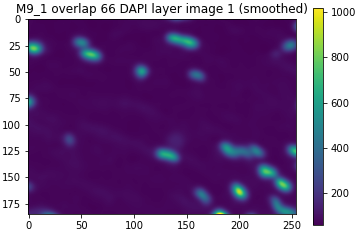
\includegraphics[width=0.49\textwidth]{images/methods/smoothed_M9_1_overlap_66_dapi_image_1}
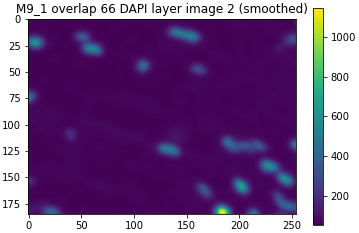
\includegraphics[width=0.49\textwidth]{images/methods/smoothed_M9_1_overlap_66_dapi_image_2}
\caption{\footnotesize First layer of the 66th overlap region in the \texttt{M9\_1} sample, after smoothing by a 3 pixel-wide Gaussian filter. The image layer on the left was exposed for 35.0 ms, and the image layer on the right was exposed for 30.0 ms.}
\label{fig:smoothed_M9_1_overlap_66}
\end{figure}

Another known quantitative difference between the two overlapping image regions is systematic and spatially-dependent variation in the illumination of each HPF. This effect, colloquially called ``flatfielding,'' is particularly important because the overlapping regions come from different portions of the two HPFs: for example, the left-hand side of one image overlaps with the right-hand side of another, and the two sides of the images are overall illuminated differently. Flatfielding, and the method for deriving correction factors for it, are discussed in \cite{flatfielding_note}, and the relevant corrections for each microscope are applied to each HPF. The only difference between the applied corrections and those derived using the full procedure in \cite{flatfielding_note} is that the masking procedure is skipped, as corrections for differences in exposure time are integral to estimation of the background thresholds and therefore the determinations of the tissue region masks. 

\reffig{fig:applied_flatfield_layers_vectra} shows examples of the flatfielding corrections applied to HPFs imaged with the Vectra 3.0 microscope for the first, middle, and last layers in each broadband filter region. Figures~\ref{fig:applied_flatfield_layers_polaris_1} and \ref{fig:applied_flatfield_layers_polaris_2} show the same, except for the corrections applied to HPFs imaged with the Vectra Polaris microscope. \reffig{fig:smoothed_flatfielded_M9_1_overlap_66} shows the same example overlapping image regions as in \reffig{fig:smoothed_M9_1_overlap_66} after application of the flatfield corrections.

\begin{figure}[!ht]
\centering
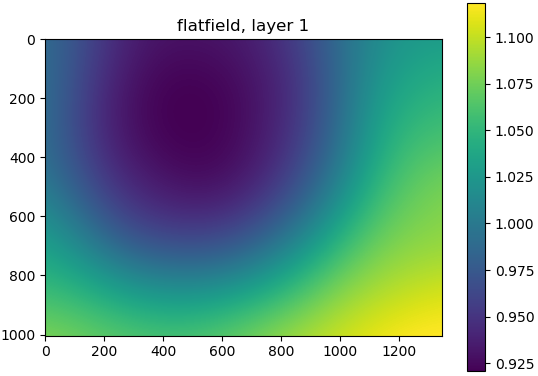
\includegraphics[width=0.3\textwidth]{images/methods/flatfield_layers_vectra/flatfield_layer_1}
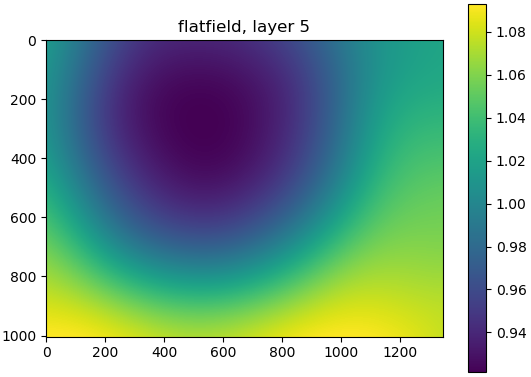
\includegraphics[width=0.3\textwidth]{images/methods/flatfield_layers_vectra/flatfield_layer_5}
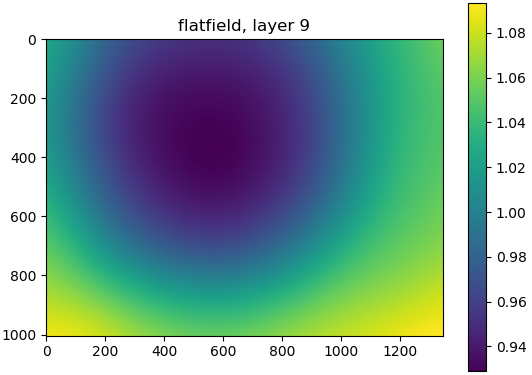
\includegraphics[width=0.3\textwidth]{images/methods/flatfield_layers_vectra/flatfield_layer_9}
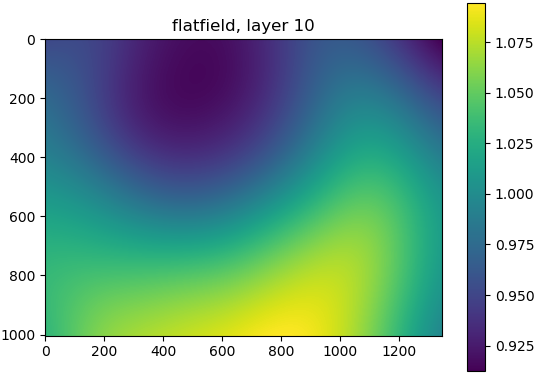
\includegraphics[width=0.3\textwidth]{images/methods/flatfield_layers_vectra/flatfield_layer_10}
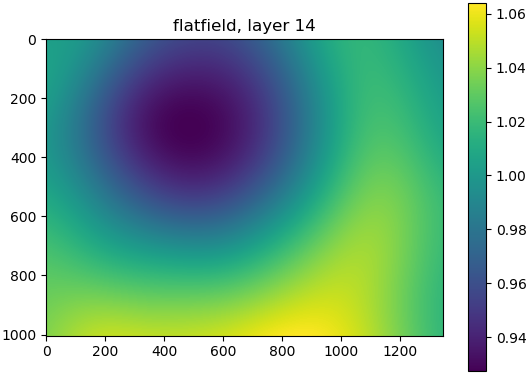
\includegraphics[width=0.3\textwidth]{images/methods/flatfield_layers_vectra/flatfield_layer_14}
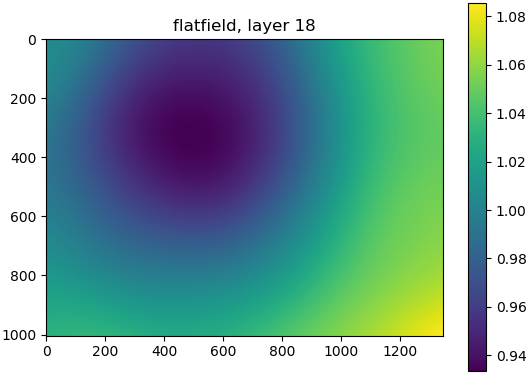
\includegraphics[width=0.3\textwidth]{images/methods/flatfield_layers_vectra/flatfield_layer_18}
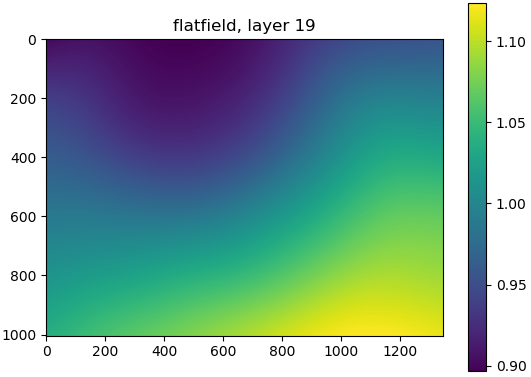
\includegraphics[width=0.3\textwidth]{images/methods/flatfield_layers_vectra/flatfield_layer_19}
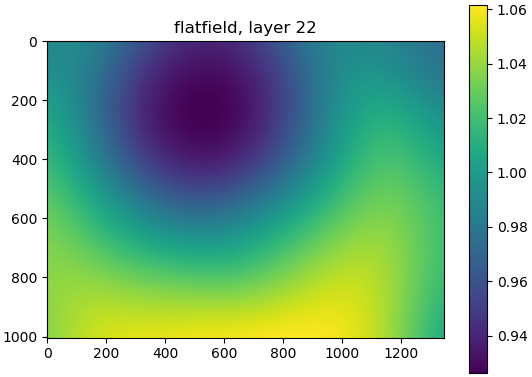
\includegraphics[width=0.3\textwidth]{images/methods/flatfield_layers_vectra/flatfield_layer_22}
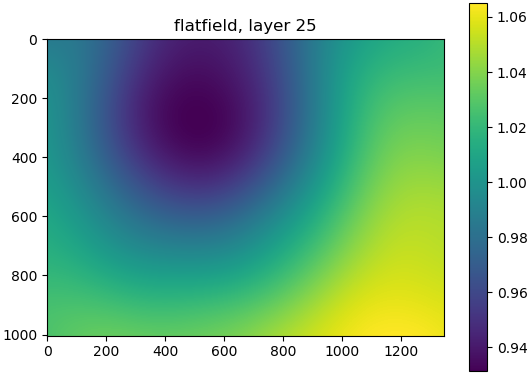
\includegraphics[width=0.3\textwidth]{images/methods/flatfield_layers_vectra/flatfield_layer_25}
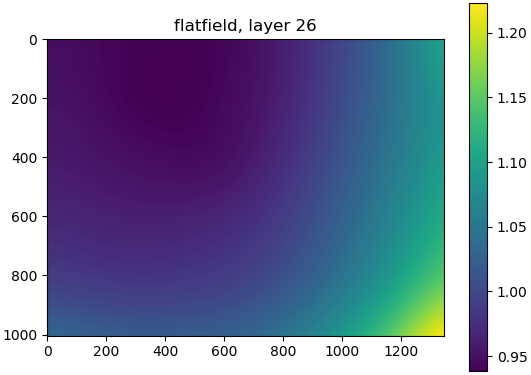
\includegraphics[width=0.3\textwidth]{images/methods/flatfield_layers_vectra/flatfield_layer_26}
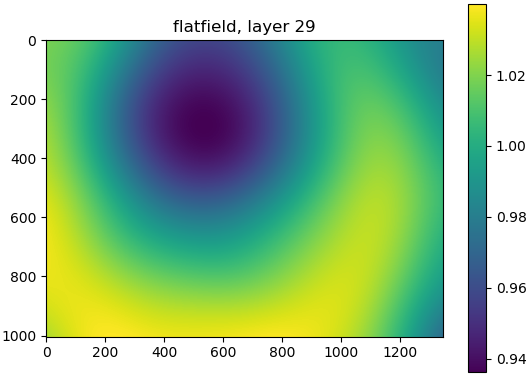
\includegraphics[width=0.3\textwidth]{images/methods/flatfield_layers_vectra/flatfield_layer_29}
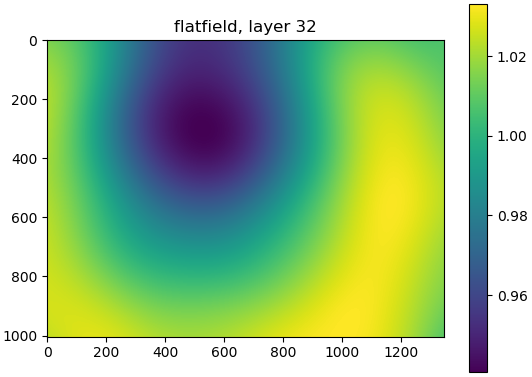
\includegraphics[width=0.3\textwidth]{images/methods/flatfield_layers_vectra/flatfield_layer_32}
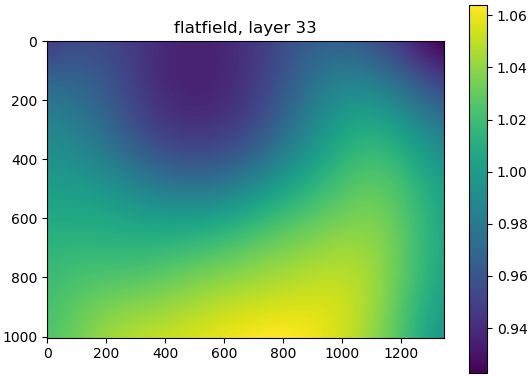
\includegraphics[width=0.3\textwidth]{images/methods/flatfield_layers_vectra/flatfield_layer_33}
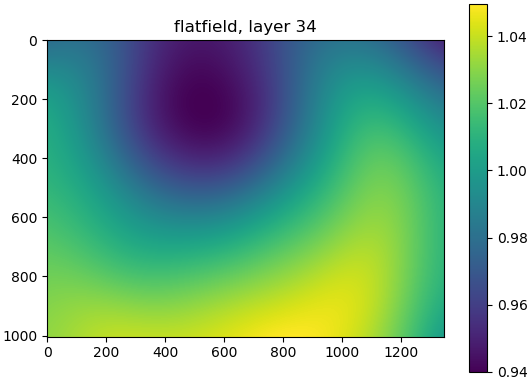
\includegraphics[width=0.3\textwidth]{images/methods/flatfield_layers_vectra/flatfield_layer_34}
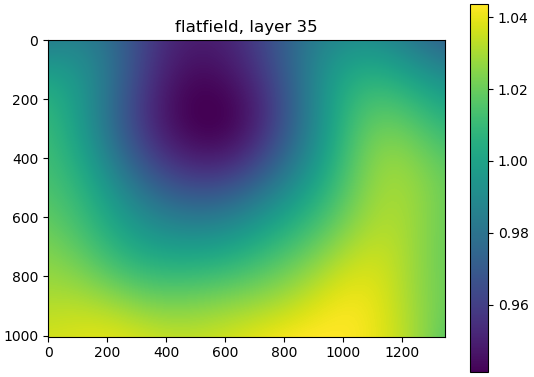
\includegraphics[width=0.3\textwidth]{images/methods/flatfield_layers_vectra/flatfield_layer_35}
\caption{\footnotesize Flatfield correction factors applied to HPFs imaged with the Vectra 3.0 microscope in layers 1, 5, 9, 10, 14, 18, 29, 22, 25, 26, 29, 32, 33, 34, and 35, from upper left to lower right, respectively.}
\label{fig:applied_flatfield_layers_vectra}
\end{figure}

\begin{figure}[!ht]
\centering
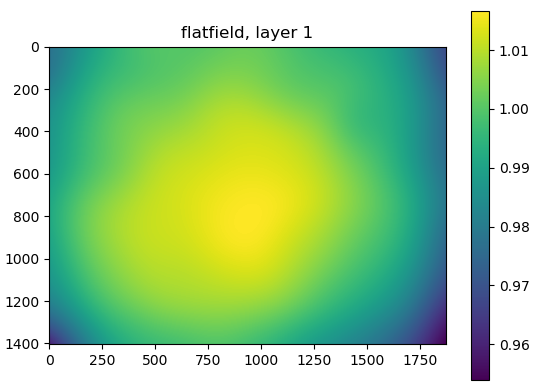
\includegraphics[width=0.3\textwidth]{images/methods/flatfield_layers_polaris/flatfield_layer_1}
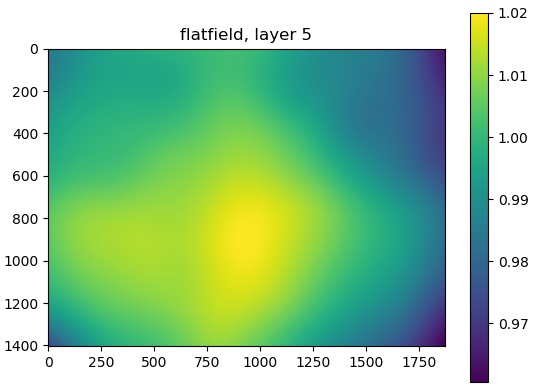
\includegraphics[width=0.3\textwidth]{images/methods/flatfield_layers_polaris/flatfield_layer_5}
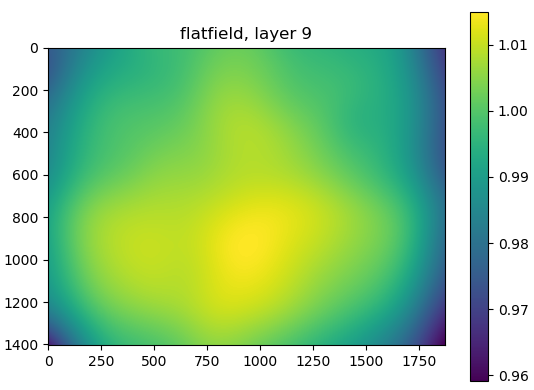
\includegraphics[width=0.3\textwidth]{images/methods/flatfield_layers_polaris/flatfield_layer_9}
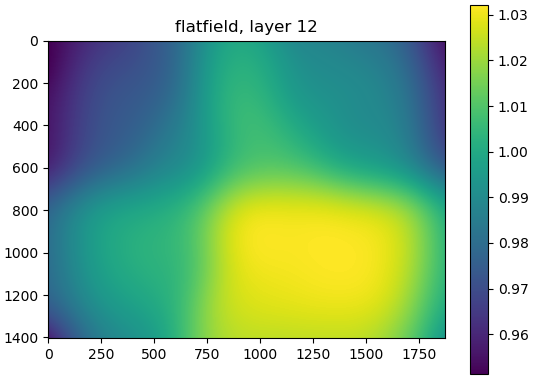
\includegraphics[width=0.3\textwidth]{images/methods/flatfield_layers_polaris/flatfield_layer_12}
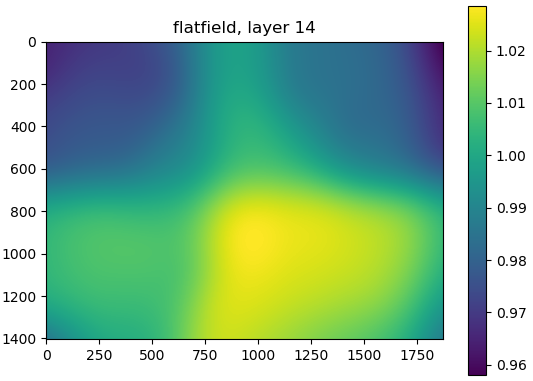
\includegraphics[width=0.3\textwidth]{images/methods/flatfield_layers_polaris/flatfield_layer_14}
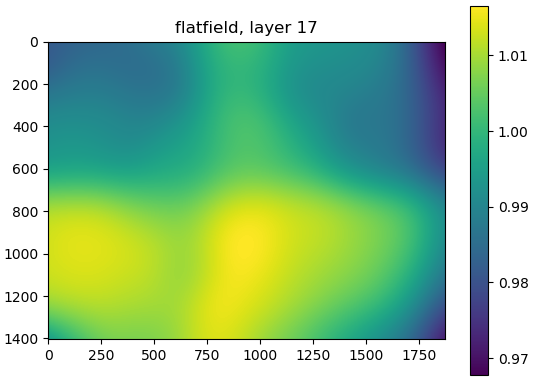
\includegraphics[width=0.3\textwidth]{images/methods/flatfield_layers_polaris/flatfield_layer_17}
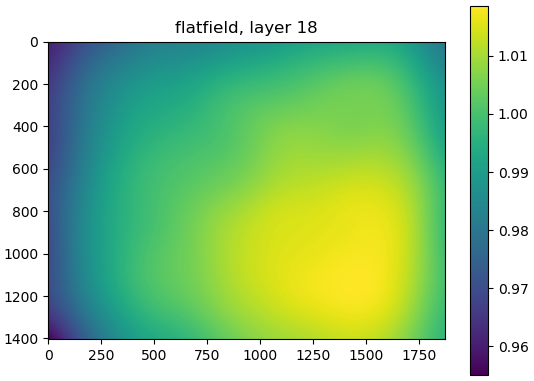
\includegraphics[width=0.3\textwidth]{images/methods/flatfield_layers_polaris/flatfield_layer_18}
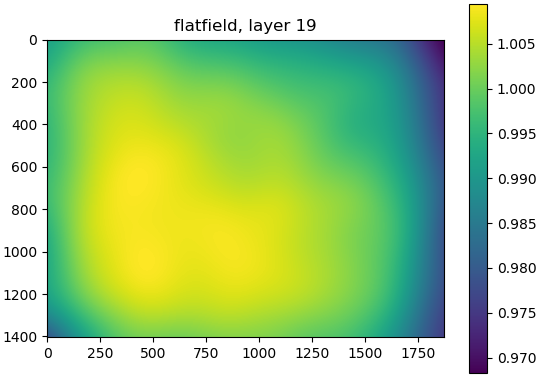
\includegraphics[width=0.3\textwidth]{images/methods/flatfield_layers_polaris/flatfield_layer_19}
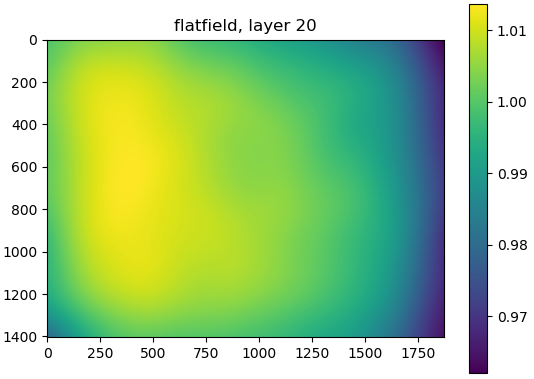
\includegraphics[width=0.3\textwidth]{images/methods/flatfield_layers_polaris/flatfield_layer_20}
\caption{\footnotesize Flatfield correction factors applied to HPFs imaged with the Vectra Polaris microscope in layers 1, 5, 9, 12, 14, 17, 18, 19, and 20, from upper left to lower right, respectively.}
\label{fig:applied_flatfield_layers_polaris_1}
\end{figure}

\begin{figure}[!ht]
\centering
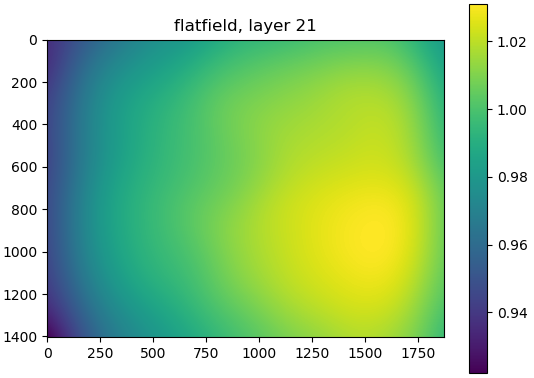
\includegraphics[width=0.3\textwidth]{images/methods/flatfield_layers_polaris/flatfield_layer_21}
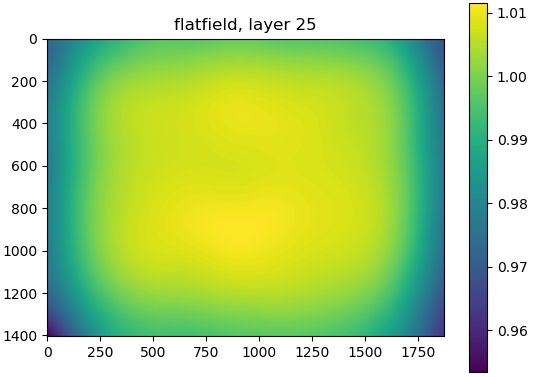
\includegraphics[width=0.3\textwidth]{images/methods/flatfield_layers_polaris/flatfield_layer_25}
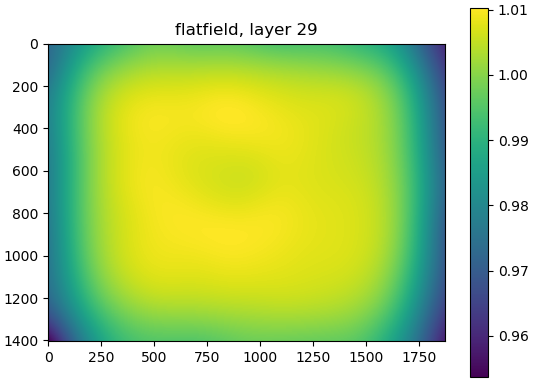
\includegraphics[width=0.3\textwidth]{images/methods/flatfield_layers_polaris/flatfield_layer_29}
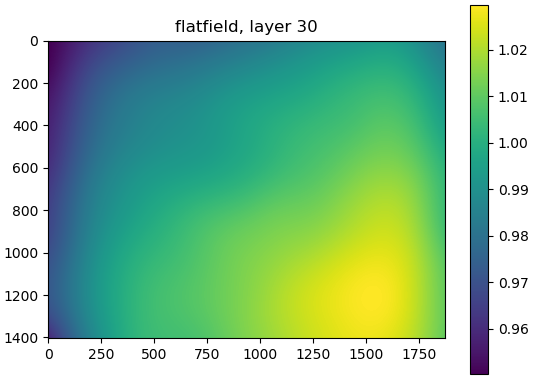
\includegraphics[width=0.3\textwidth]{images/methods/flatfield_layers_polaris/flatfield_layer_30}
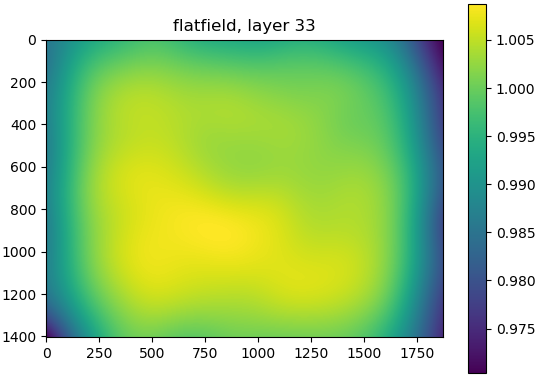
\includegraphics[width=0.3\textwidth]{images/methods/flatfield_layers_polaris/flatfield_layer_33}
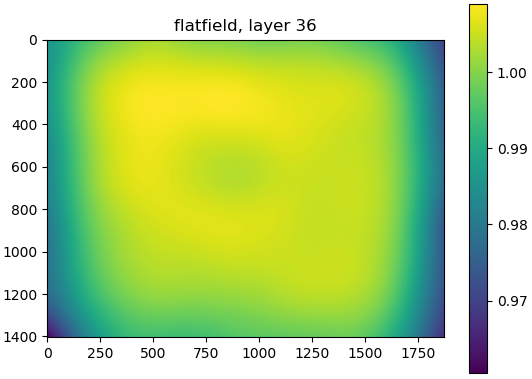
\includegraphics[width=0.3\textwidth]{images/methods/flatfield_layers_polaris/flatfield_layer_36}
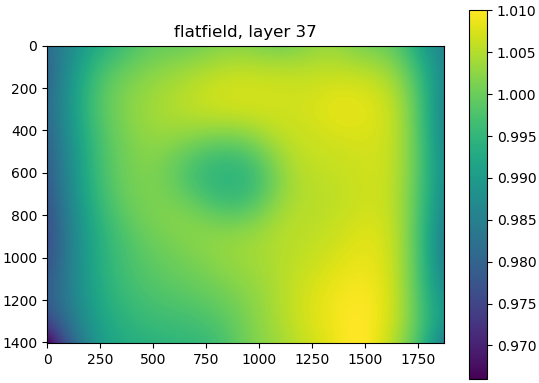
\includegraphics[width=0.3\textwidth]{images/methods/flatfield_layers_polaris/flatfield_layer_37}
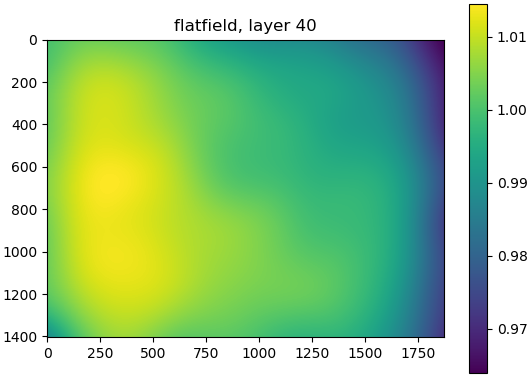
\includegraphics[width=0.3\textwidth]{images/methods/flatfield_layers_polaris/flatfield_layer_40}
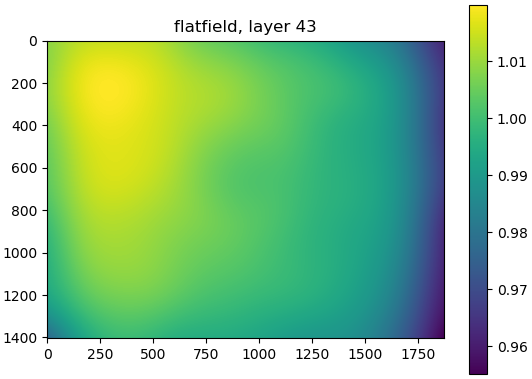
\includegraphics[width=0.3\textwidth]{images/methods/flatfield_layers_polaris/flatfield_layer_43}
\caption{\footnotesize Flatfield correction factors applied to HPFs imaged with the Vectra Polaris microscope in layers 21, 25, 29, 30, 33, 36, 37, 40, and 43, from upper left to lower right, respectively.}
\label{fig:applied_flatfield_layers_polaris_2}
\end{figure}

\begin{figure}[!ht]
\centering
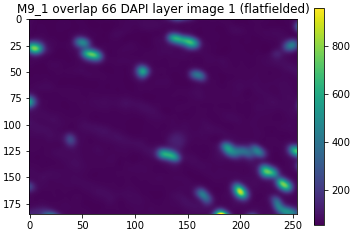
\includegraphics[width=0.49\textwidth]{images/methods/smoothed_flatfielded_M9_1_overlap_66_dapi_image_1}
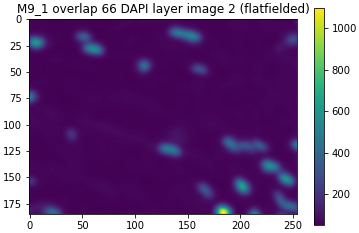
\includegraphics[width=0.49\textwidth]{images/methods/smoothed_flatfielded_M9_1_overlap_66_dapi_image_2}
\caption{\footnotesize First layer of the 66th overlap region in the \texttt{M9\_1} sample, after smoothing by a 3 pixel-wide Gaussian filter and application of flatfield correction factors. The image layer on the left was exposed for 35.0 ms, and the image layer on the right was exposed for 30.0 ms.}
\label{fig:smoothed_flatfielded_M9_1_overlap_66}
\end{figure}

Next, while the spatial extents of the overlapping regions (i.e. the exact subsets of the total images to use) are technically defined by the 20\% boundaries around each HPF, there are often minute relative translations of the microscope stage that occur between imaging of individual HPFs that makes these boundaries imperfect at the scale of a few pixels. The registrations of these image regions to a shared local coordinate system must therefore be performed using the pair-wise alignment procedure discussed in \cite{Heshy} to ensure the image regions in each overlap aren't translated relative to one another. 

\reffig{fig:smoothed_flatfielded_aligned_M9_1_overlap_66} shows the same image regions as in \reffig{fig:smoothed_flatfielded_M9_1_overlap_66} after they have been pairwise aligned. In addition to showing the two image layer regions separately, \reffig{fig:smoothed_flatfielded_aligned_M9_1_overlap_66} also shows them overlaid on one another in a false color image, where the HPF on the left hand side is colored magenta and the other is colored green, so that the resulting overlay appears white when the two image contents are identical and more magenta or green when one image is brighter than the other. In this example, the false color overlay appears magenta overall in color because the left-hand image was exposed for longer.

\begin{figure}[!ht]
\centering
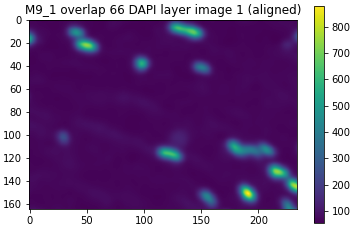
\includegraphics[width=0.49\textwidth]{images/methods/smoothed_flatfielded_aligned_M9_1_overlap_66_dapi_image_1}
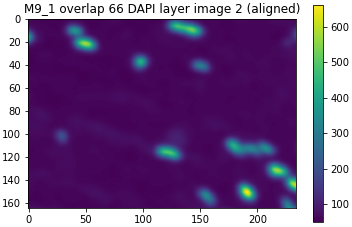
\includegraphics[width=0.49\textwidth]{images/methods/smoothed_flatfielded_aligned_M9_1_overlap_66_dapi_image_2}
\includegraphics[width=0.49\textwidth]{images/methods/smoothed_flatfielded_aligned_M9_1_overlap_66_dapi_overlay}
\caption{\footnotesize Upper: first layer of the 66th overlap region in the \texttt{M9\_1} sample, after smoothing by a 3 pixel-wide Gaussian filter, application of flatfield correction factors, and small relative translations determined by pairwise alignment. The image layer on the left was exposed for 35.0 ms, and the image layer on the right was exposed for 30.0 ms. Lower: false color overlay of the two images in the upper part of the figure, where the left-hand image is colored magenta and the right hand image in colored green.}
\label{fig:smoothed_flatfielded_aligned_M9_1_overlap_66}
\end{figure}

Finally, a last known difference between the overlap images is spatially-dependent ``warping'' effects introduced by the microscope camera. The exact warping patterns can only be measured following precise corrections for exposure time differences and flatfielding, but it is known that the effects are generally largest on the edges of each HPF. Therefore, the spatial extent of each overlapping region in the local coordinate system is restricted to the central 50\% in each of the height and width dimensions, and only about 25\% of the total overlapping area is used in each pair of images. \reffig{fig:smoothed_flatfielded_aligned_clipped_M9_1_overlap_66} shows the final images used to calculate the cost from the 66th overlap in \texttt{M9\_1}, after all corrections are applied and the outer 75\% of each image is cut out, as well as the false color overlay of the two images. The predominant remaining difference in the images (as is visible in the false color overlay) is the overall scale of illumination due to the differences in exposure times. 

\begin{figure}[!ht]
\centering
\includegraphics[width=0.49\textwidth]{images/methods/smoothed_flatfielded_aligned_clipped_M9_1_overlap_66_dapi_image_1}
\includegraphics[width=0.49\textwidth]{images/methods/smoothed_flatfielded_aligned_clipped_M9_1_overlap_66_dapi_image_2}
\includegraphics[width=0.49\textwidth]{images/methods/smoothed_flatfielded_aligned_clipped_M9_1_overlap_66_dapi_overlay}
\caption{\footnotesize Upper: first layer of the 66th overlap region in the \texttt{M9\_1} sample, after smoothing by a 3 pixel-wide Gaussian filter, application of flatfield correction factors and alignment shifts, and removal of the outer (lower left) 75\% portions of each image. The image layer on the left was exposed for 35.0 ms, and the image layer on the right was exposed for 30.0 ms. Lower: false color overlay of the two images in the upper part of the figure, where the left-hand image is colored magenta and the right hand image in colored green.}
\label{fig:smoothed_flatfielded_aligned_clipped_M9_1_overlap_66}
\end{figure}

The slides used in each layer group are those that have at least 1500 overlaps with differing HPF exposure times, after neglecting any overlaps where at least one HPF is located on the edge of the slide's tissue region (to minimize the amount of empty background included), and only counting overlaps that are bright and distinct enough to be pairwise-aligned. Up to ten slides are used in each layer group, sorted by the number of overlaps they contribute. \reffig{fig:n_overlaps_used_vectra} shows the numbers of overlaps used to independently estimate the dark current for each sample in each layer for the slides collected using the Vectra 3.0 microscope, and \reffig{fig:n_overlaps_used_polaris} shows the same for the slides collected with the Vectra Polaris microscope. Layers 10 and 11 in the Vectra Polaris slides were all recorded with identical exposure times, and so no estimates of the dark current offsets can (or must) be made for those layers. 

\begin{figure}[!ht]
\centering
\includegraphics[width=0.95\textwidth]{images/methods/n_overlaps_used_vectra}
\caption{\footnotesize Number of overlaps used from each sample to determine the dark current in each image layer for images collected with the Vectra 3.0 microscope. The thick dotted black lines separate layers imaged with different filter cubes.}
\label{fig:n_overlaps_used_vectra}
\end{figure}

\begin{figure}[!ht]
\centering
\includegraphics[width=0.95\textwidth]{images/methods/n_overlaps_used_polaris}
\caption{\footnotesize Number of overlaps used from each sample to determine the dark current in each image layer for images collected with the Vectra Polaris microscope. The thick dotted black lines separate layers imaged with different filter cubes. Layers 10 and 11 of every image have the same exposure time, so no estimate of the dark current is made for those layers. }
\label{fig:n_overlaps_used_polaris}
\end{figure}

Theoretically, there should not be any pixels in any image observed with a number of counts less than the constant noise from the dark current, but this is not the case in practice due to random noise and Poisson count error. This possible undercounting is the reason for the cases with $I^{ijm}_{1} \leq D^{m}$ and $I^{ijm}_{1} \leq D^{m}$ in \refeq{eq:image_corr_def_1} and \refeq{eq:image_corr_def_2}, but these cases may also bias the minimization results toward larger values of $D^{m}$. To prevent any bias, then, an upper bound is set on the allowed values of $D^{m}$ for the minimization in each sample and layer. This upper bound is set at the smallest integer value for which more than 0.01\% of the pixels in any image have counts less than the upper bound.

Calculating the cost of any individual overlap as defined in \refeq{eq:minimization_def} requires comparing every pair of individual pixel values, which consumes a significant amount of computational memory when a large number of overlaps is used in the minimization. To reduce the amount of memory required, the cost from each individual overlap is calculated from a pre-determined curve, instead of from the image pixel contents, during minimization. Each overlap's true cost is calculated as the images are first read in at 100 evenly-spaced values between zero and the upper bound on $D$, and then during minimization the cost is calculated by linearly interpolating between the nearest points on that predetermined curve. 

Figures ~\ref{fig:overlap_cost_examples_vectra_1}-\ref{fig:overlap_cost_examples_polaris_2} show some examples of individual overlap false color overlay comparisons before and after correction with the optimal $D$ found for their particular sample layer, along with their associated costs between the fitting bounds as calculated from the unsmoothed/flatfielded whole images and from the smoothed/flatfielded aligned central region-only images. Figures~\ref{fig:overlap_cost_examples_vectra_1} and \ref{fig:overlap_cost_examples_vectra_2} show some examples for samples imaged with the Vectra 3.0 microscope, and Figures~\ref{fig:overlap_cost_examples_polaris_1} and \ref{fig:overlap_cost_examples_polaris_2} show examples for samples imaged with the Vectra Polaris microscope. The overlays give a qualitative idea of how applying corrections for differences in exposure time affects comparisons between the overlapping image regions.

\begin{figure}[!ht]
\centering
\includegraphics[width=0.95\textwidth]{images/methods/cost_examples_vectra/overlay_comp_random_6761_offset=18.961}
\includegraphics[width=0.95\textwidth]{images/methods/cost_examples_vectra/overlay_comp_random_2425_offset=20.326}
\includegraphics[width=0.95\textwidth]{images/methods/cost_examples_vectra/overlay_comp_random_3946_offset=20.222}
\caption{\footnotesize Left and center columns: false color overlay comparisons before (left column) and after (center column) correction for differences in exposure times with the optimal $D^{m}$ determined from the minimization in \refeq{eq:minimization_def} for several sample layers imaged using the Vectra 3.0 microscope. The overlays show the full overlap region without smoothing, but the costs above them are calculated with the smoothed central regions of the overlaps. Right column: L1-norm costs for the same overlaps at 100 values of $D$ between zero and the sample/layer-dependent upper bound. Costs calculated using the entire unsmoothed image regions are shown in blue, and costs calculated from the smoothed central image regions are shown in orange. In both cases corrections for flatfielding are applied and the images are pairwise-aligned. The vertical black line shows the best-fit value of $D$ for each overlap's sample and layer. The differences in image exposure times are given in milliseconds. From the upper to lower rows, the overlaps shown are examples from layer 1 of \texttt{M26\_1}, layer 10 of \texttt{M17\_1}, and layer 23 of \texttt{M3\_1}, respectively.}
\label{fig:overlap_cost_examples_vectra_1}
\end{figure}

\begin{figure}[!ht]
\centering
\includegraphics[width=0.95\textwidth]{images/methods/cost_examples_vectra/overlay_comp_random_10478_offset=17.778}
\includegraphics[width=0.95\textwidth]{images/methods/cost_examples_vectra/overlay_comp_random_892_offset=21.314}
\caption{\footnotesize Left and center columns: false color overlay comparisons before (left column) and after (center column) correction for differences in exposure times with the optimal $D^{m}$ determined from the minimization in \refeq{eq:minimization_def} for several sample layers imaged using the Vectra 3.0 microscope. The overlays show the full overlap region without smoothing, but the costs above them are calculated with the smoothed central regions of the overlaps. Right column: L1-norm costs for the same overlaps at 100 values of $D$ between zero and the sample/layer-dependent upper bound. Costs calculated using the entire unsmoothed image regions are shown in blue, and costs calculated from the smoothed central image regions are shown in orange. In both cases corrections for flatfielding are applied and the images are pairwise-aligned. The vertical black line shows the best-fit value of $D$ for each overlap's sample and layer. The differences in image exposure times are given in milliseconds. In the upper and lower rows the overlaps shown are examples from layer 31 of \texttt{M51\_1} and layer 33 of \texttt{M4\_2}, respectively.}
\label{fig:overlap_cost_examples_vectra_2}
\end{figure}

\begin{figure}[!ht]
\centering
\includegraphics[width=0.95\textwidth]{images/methods/cost_examples_polaris/overlay_comp_random_4357_offset=51.980}
\includegraphics[width=0.95\textwidth]{images/methods/cost_examples_polaris/overlay_comp_random_2668_offset=51.848}
\includegraphics[width=0.95\textwidth]{images/methods/cost_examples_polaris/overlay_comp_random_1554_offset=51.000}
\caption{\footnotesize Left and center columns: false color overlay comparisons before (left column) and after (center column) correction for differences in exposure times with the optimal $D^{m}$ determined from the minimization in \refeq{eq:minimization_def} for several sample layers imaged using the Vectra Polaris microscope. The overlays show the full overlap region without smoothing, but the costs above them are calculated with the smoothed central regions of the overlaps. Right column: L1-norm costs for the same overlaps at 100 values of $D$ between zero and the sample/layer-dependent upper bound. Costs calculated using the entire unsmoothed image regions are shown in blue, and costs calculated from the smoothed central image regions are shown in orange. In both cases corrections for flatfielding are applied and the images are pairwise-aligned. The vertical black line shows the best-fit value of $D$ for each overlap's sample and layer. The differences in image exposure times are given in milliseconds. From the upper to lower rows, the overlaps shown are examples from layer 4 of \texttt{YX10}, layer 16 of \texttt{PZ29}, and layer 19 of \texttt{YY15}, respectively.}
\label{fig:overlap_cost_examples_polaris_1}
\end{figure}

\begin{figure}[!ht]
\centering
\includegraphics[width=0.95\textwidth]{images/methods/cost_examples_polaris/overlay_comp_random_5023_offset=50.770}
\includegraphics[width=0.95\textwidth]{images/methods/cost_examples_polaris/overlay_comp_random_4697_offset=49.636}
\includegraphics[width=0.95\textwidth]{images/methods/cost_examples_polaris/overlay_comp_random_1916_offset=50.424}
\caption{\footnotesize Left and center columns: false color overlay comparisons before (left column) and after (center column) correction for differences in exposure times with the optimal $D^{m}$ determined from the minimization in \refeq{eq:minimization_def} for several sample layers imaged using the Vectra Polaris microscope. The overlays show the full overlap region without smoothing, but the costs above them are calculated with the smoothed central regions of the overlaps. Right column: L1-norm costs for the same overlaps at 100 values of $D$ between zero and the sample/layer-dependent upper bound. Costs calculated using the entire unsmoothed image regions are shown in blue, and costs calculated from the smoothed central image regions are shown in orange. In both cases corrections for flatfielding are applied and the images are pairwise-aligned. The vertical black line shows the best-fit value of $D$ for each overlap's sample and layer. The differences in image exposure times are given in milliseconds. From the upper to lower rows, the overlaps shown are examples from layer 24 of \texttt{YZ68}, layer 31 of \texttt{YY15}, and layer 40 of \texttt{PZ14}, respectively.}
\label{fig:overlap_cost_examples_polaris_2}
\end{figure}

\reffig{fig:cost_reduction_plots_M51_1_layer_30} shows a typical example (for the 30th layer of the Vectra 3.0 sample \texttt{M51\_1}) of how the costs from all the individual overlaps change as a result of applying corrections for exposure time differences with the best-fit $D$ found for this sample. Before correction, a clear correlation is visible between the difference in an overlap's image exposure times and its cost. This correlation is not present after correction. \reffig{fig:cost_reduction_plots_YZ68_layer_12} shows the same for the 12th layer of the Vectra Polaris sample \texttt{YZ68}.

\begin{figure}[!ht]
\centering
\includegraphics[width=0.95\textwidth]{images/methods/cost_reduction_plots_2d_M51_1_layer_30}
\caption{\footnotesize Two-dimensional histograms of pre-fit cost (upper left), post-fit cost (upper right), cost reduction (pre-fit minus post-fit cost) (lower left), and fractional cost reduction (cost reduction divided by pre-fit cost) (lower right) vs. difference in image exposure times for all overlaps used in the minimization for layer 30 of the Vectra 3.0 sample \texttt{M51\_1}.}
\label{fig:cost_reduction_plots_M51_1_layer_30}
\end{figure}

\begin{figure}[!ht]
\centering
\includegraphics[width=0.95\textwidth]{images/methods/cost_reduction_plots_2d_YZ68_layer_12}
\caption{\footnotesize Two-dimensional histograms of pre-fit cost (upper left), post-fit cost (upper right), cost reduction (pre-fit minus post-fit cost) (lower left), and fractional cost reduction (cost reduction divided by pre-fit cost) (lower right) vs. difference in image exposure times for all overlaps used in the minimization for layer 12 of the Vectra Polaris sample \texttt{YZ68}.}
\label{fig:cost_reduction_plots_YZ68_layer_12}
\end{figure}

\clearpage

%%%%%%%%%%%%%%%%%%%%%%%%%%%%%%%%%%%%%%%%%%%%%% RESULTS SECTION %%%%%%%%%%%%%%%%%%%%%%%%%%%%%%%%%%%%%%%%%%%%%%
\section{Results}
\label{sec:results}

The optimal dark current offsets found for each sample used are pictured in \reffig{fig:dark_current_offsets_vectra} for the 35 layers of the Vectra 3.0 samples, and in \reffig{fig:dark_current_offsets_polaris} for the 43 layers of the Vectra Polaris samples. The figures also show the final weighted average dark current offsets in each layer in black, and these values are also listed in \reftab{tab:best_offsets_vectra} for the Vectra 3.0 samples and in \reftab{tab:best_offsets_polaris} for the Vectra Polaris samples. The values found for the individual samples and overall are all very similar, but there is some dependence on the image layer, particularly for layers near the extremes of the broadband filter groups. Generally, the dark current offsets found for the Vectra Polaris samples are higher than those for the Vectra 3.0 samples.

\begin{figure}[!ht]
\centering
\includegraphics[width=0.95\textwidth]{images/results/dark_current_offsets_vectra}
\caption{\footnotesize Optimal dark current offsets found independently for each sample (dashed lines) and the overall weighted averages (solid black lines/points) in each layer for images collected with the Vectra 3.0 microscope. The thick dotted black lines separate layers imaged with different filter cubes.}
\label{fig:dark_current_offsets_vectra}
\end{figure}

\begin{table}[!htb]
\centering
\begin{tabular}{c c c}
Image layer & Number of overlaps & Overall best $D$ \\
\hline
1           & 75706              & 19.07 \\
2           & 75824              & 19.18 \\
3           & 75802              & 19.35 \\
4           & 75758              & 19.57 \\
5           & 75770              & 18.68 \\
6           & 75766              & 18.28 \\
7           & 75758              & 17.98 \\
8           & 75748              & 17.82 \\
9           & 75740              & 17.86 \\
10          & 49698              & 20.22 \\
11          & 49724              & 20.42 \\
12          & 49694              & 19.37 \\
13          & 49674              & 18.19 \\
14          & 49640              & 17.88 \\
15          & 49628              & 17.82 \\
16          & 49614              & 17.83 \\
17          & 49598              & 17.85 \\
18          & 49546              & 17.85 \\
19          & 37340              & 19.41 \\
20          & 37392              & 20.57 \\
21          & 37414              & 19.81 \\
22          & 37412              & 19.63 \\
23          & 37414              & 19.74 \\
24          & 37386              & 19.40 \\
25          & 37354              & 18.97 \\
26          & 57094              & 16.87 \\
27          & 60780              & 17.83 \\
28          & 61010              & 17.87 \\
29          & 61036              & 17.89 \\
30          & 61032              & 17.90 \\
31          & 60926              & 17.84 \\
32          & 60816              & 17.83 \\
33          & 13022              & 20.77 \\
34          & 13022              & 20.83 \\
35          & 13018              & 19.65 \\
\hline
\end{tabular}
\caption{\footnotesize Total number of overlaps used in minimization, and final pixel-weighted averages of best-fit dark current offsets in each layer ($D$), for HPFs imaged using the Vectra 3.0 microscope.}
\label{tab:best_offsets_vectra}
\end{table}

\begin{figure}[!ht]
\centering
\includegraphics[width=0.95\textwidth]{images/results/dark_current_offsets_polaris}
\caption{\footnotesize Optimal dark current offsets found independently for each sample (dashed lines) and the overall weighted averages (solid black lines/points) in each layer for images collected with the Vectra Polaris microscope. The thick dotted black lines separate layers imaged with different filter cubes. Layers 10 and 11 of every image have the same exposure time, so no estimate of the dark current is made for those layers.}
\label{fig:dark_current_offsets_polaris}
\end{figure}

\begin{table}[!htb]
\centering
\begin{tabular}{c c c}
Image layer & Number of overlaps & Overall best $D$ \\
\hline
1           & 8944               & 56.55 \\
2           & 8944               & 60.15 \\
3           & 8944               & 60.41 \\
4           & 8942               & 59.02 \\
5           & 8942               & 57.43 \\
6           & 8942               & 55.92 \\
7           & 8944               & 54.06 \\
8           & 8942               & 53.08 \\
9           & 8942               & 51.31 \\
12          & 53598              & 49.76 \\
13          & 53690              & 52.44 \\
14          & 53702              & 54.76 \\
15          & 53706              & 56.19 \\
16          & 53724              & 56.25 \\
17          & 53760              & 55.11 \\
18          & 3416               & 51.01 \\
19          & 3416               & 52.52 \\
20          & 3416               & 52.01 \\
21          & 33336              & 50.06 \\
22          & 33452              & 50.60 \\
23          & 33474              & 50.52 \\
24          & 33470              & 50.26 \\
25          & 33458              & 50.37 \\
26          & 33446              & 50.14 \\
27          & 33446              & 50.43 \\
28          & 33440              & 50.47 \\
29          & 33422              & 50.70 \\
30          & 35330              & 49.84 \\
31          & 35386              & 50.65 \\
32          & 35374              & 50.53 \\
33          & 35350              & 50.56 \\
34          & 35346              & 50.29 \\
35          & 35330              & 50.51 \\
36          & 35300              & 50.48 \\
37          & 18596              & 50.00 \\
38          & 22158              & 50.19 \\
39          & 22214              & 50.99 \\
40          & 22262              & 50.80 \\
41          & 22272              & 50.24 \\
42          & 22256              & 50.01 \\
43          & 22210              & 49.71 \\
\hline
\end{tabular}
\caption{\footnotesize Total number of overlaps used in minimization, and final pixel-weighted averages of best-fit dark current offsets in each layer ($D$), for HPFs imaged using the Vectra Polaris microscope.}
\label{tab:best_offsets_polaris}
\end{table}

\clearpage

%%%%%%%%%%%%%%%%%%%%%%%%%%%%%%%%%%%%%%%%%%%%%% SUMMARY SECTION %%%%%%%%%%%%%%%%%%%%%%%%%%%%%%%%%%%%%%%%%%%%%%
\section{Summary}
\label{sec:summary}

%%%%%%%%%%%%%%%%%%%%%%%%%%%%%%%%%%%%%%%%%%%%%%% BIBLIOGRAPHY %%%%%%%%%%%%%%%%%%%%%%%%%%%%%%%%%%%%%%%%%%%%%%%%
\clearpage
\bibliography{references}

\end{document}